\documentclass[9pt,twocolumn,twoside]{pnas-new}
% Use the lineno option to display guide line numbers if required.

\articletype{SOCIAL SCIENCES}%%%% Article topic/classification

\templatetype{pnasresearcharticle} % Choose template
\setboolean{displaywatermark}{false}

\usepackage{siunitx}
\usepackage{xurl}
% Generated by `python -m src.paper_numbers`. Do not edit by hand.
\newcommand{\nPlaylists}{50}
\newcommand{\nFunctional}{45}
\newcommand{\nGenre}{5}
\newcommand{\nSlots}{9{,}004}
\newcommand{\nTracks}{8{,}093}
\newcommand{\nNames}{5{,}024}
\newcommand{\nFal}{100{,}380}
\newcommand{\nFalIn}{63{,}266}
\newcommand{\nCovers}{8{,}056}
\newcommand{\nHouses}{486}
\newcommand{\nWithRegistrant}{3{,}446}
\newcommand{\deezerMatch}{73\%}
\newcommand{\deezerMatchF}{72\%}
\newcommand{\deezerMatchG}{94\%}
\newcommand{\fplF}{0.0025}
\newcommand{\fplG}{0.21}
\newcommand{\aliasOnlyF}{81\%}
\newcommand{\aliasOnlyG}{5\%}
\newcommand{\verifiedF}{18\%}
\newcommand{\verifiedG}{94\%}
\newcommand{\nGhost}{3{,}170}
\newcommand{\ghostShareNamesF}{70\%}
\newcommand{\refFirefly}{90\%}
\newcommand{\nFirefly}{50}
\newcommand{\refEpidemic}{10\%}
\newcommand{\nEpidemic}{40}
\newcommand{\refMajors}{18\%}
\newcommand{\nMajors}{278}
\newcommand{\refGenreNames}{3\%}
\newcommand{\nGenreNames}{493}
\newcommand{\nGenreFlagged}{14}
\newcommand{\epidemicFplRatio}{11}
\newcommand{\epidemicBio}{95\%}
\newcommand{\profGN}{3{,}156}
\newcommand{\profGHouse}{222}
\newcommand{\profGFpl}{1.4}
\newcommand{\profGAlias}{86\%}
\newcommand{\profGSelf}{55\%}
\newcommand{\profRN}{1{,}374}
\newcommand{\profRHouse}{10}
\newcommand{\profRFpl}{25}
\newcommand{\profRAlias}{45\%}
\newcommand{\profRSelf}{13\%}
\newcommand{\slotGhostF}{75\%}
\newcommand{\slotGhostG}{1\%}
\newcommand{\playsGhost}{33.7}
\newcommand{\playsReal}{13.1}
\newcommand{\ghostWithReg}{2{,}311}
\newcommand{\ghostHouses}{66}
\newcommand{\topEightGhostNames}{81\%}
\newcommand{\topEightGhostSlots}{84\%}
\newcommand{\topEightSE}{7}
\newcommand{\seGhost}{85\%}
\newcommand{\seReal}{17\%}
\newcommand{\medHouseGhost}{222}
\newcommand{\medHouseReal}{6}
\newcommand{\selfSourceGhost}{55\%}
\newcommand{\selfSourceReal}{13\%}
\newcommand{\selfSourceHouse}{264}
\newcommand{\nMultiHouse}{225}
\newcommand{\lfTopEightCodedF}{72\%}
\newcommand{\lfTopEightAllF}{52\%}
\newcommand{\lfNoCodeF}{28\%}
\newcommand{\lfTopEightCodedG}{22\%}
\newcommand{\lfHousesF}{339}
\newcommand{\lfHousesG}{197}
\newcommand{\flowRRDeg}{2.42}
\newcommand{\flowRGDeg}{0.48}
\newcommand{\flowGRDeg}{0.56}
\newcommand{\flowGGDeg}{1.16}
\newcommand{\sameDeg}{2.33}
\newcommand{\flowRRPl}{1.13}
\newcommand{\flowRGPl}{0.82}
\newcommand{\flowGRPl}{0.86}
\newcommand{\flowGGPl}{1.03}
\newcommand{\samePl}{1.37}
\newcommand{\nullRange}{4\%}
\newcommand{\sameObs}{6{,}702}
\newcommand{\sameExpPl}{4{,}881}
\newcommand{\realSlotsToGhost}{14\%}
\newcommand{\ghostSlotsToGhost}{65\%}
\newcommand{\inSetReal}{40\%}
\newcommand{\inSetGhost}{76\%}
\newcommand{\louvainQ}{0.85}
\newcommand{\louvainQnull}{0.18}
\newcommand{\nComm}{58}
\newcommand{\nGiant}{4{,}620}
\newcommand{\nmiHome}{0.70}
\newcommand{\nmiHomeNull}{0.05}
\newcommand{\nmiHouse}{0.32}
\newcommand{\nmiHouseNull}{0.15}
\newcommand{\nmiLabel}{0.15}
\newcommand{\aucName}{0.61}
\newcommand{\nName}{4{,}530}
\newcommand{\aucTitles}{0.63}
\newcommand{\nTitles}{4{,}530}
\newcommand{\aucBio}{0.89}
\newcommand{\nBio}{1{,}944}
\newcommand{\aucCover}{0.75}
\newcommand{\nCover}{4{,}072}
\newcommand{\aucAudio}{0.52}
\newcommand{\nAudio}{624}
\newcommand{\aucBioLength}{0.80}
\newcommand{\nAudioPlaylists}{40}
\newcommand{\bioGhost}{22\%}
\newcommand{\bioReal}{91\%}
\newcommand{\entGhost}{43\%}
\newcommand{\entReal}{88\%}
\newcommand{\tokGhost}{32}
\newcommand{\tokReal}{146}
\newcommand{\personGhost}{58\%}
\newcommand{\personRealF}{58\%}
\newcommand{\coverSameHouse}{15\%}
\newcommand{\coverSameHouseNull}{6\%}

\graphicspath{{figures/}{../figures/}} % figures/ on Overleaf, ../figures/ locally

% Course hand-in, not a submission: no line numbers (watermark is off above).
\makeatletter
\def\PNAS@linecountLO{}\def\PNAS@linecountRO{}\def\PNAS@linecountLE{}\def\PNAS@linecountRE{}
\def\PNAS@linecountsecpageLO{}\def\PNAS@linecountsecpageRO{}\def\PNAS@linecountsecpageLE{}\def\PNAS@linecountsecpageRE{}
% First page: run the class's firststyle (it allocates the line-count boxes,
% so it must not be replaced), then drop its line numbers and journal footer.
\let\PNAS@origfirststyle\ps@firststyle
\def\ps@firststyle{\PNAS@origfirststyle\fancyhead{}%
  \fancyfoot[L]{\footerfont 02805 Social Graphs and Interactions\hspace{7pt}|\hspace{7pt}November 2026}
  \fancyfoot[R]{\footerfont\textbf{\thepage\ of \pageref*{LastPage}}}}
\makeatother

% Footer on pages 2+: course instead of journal placeholders.
\fancyfoot[RO]{\footerfont 02805 Social Graphs and Interactions\hspace{7pt}|\hspace{7pt}November 2026\hspace{7pt}|\hspace{7pt}\textbf{\thepage}}
\fancyfoot[LO]{}
\fancyfoot[RE]{}
\fancyfoot[LE]{\footerfont\textbf{\thepage}\hspace{7pt}|\hspace{7pt}02805 Social Graphs and Interactions\hspace{7pt}|\hspace{7pt}November 2026}

\begin{document}

\title{Many faces, few hands. How credit networks reveal Spotify's ghost artists, and where the recommender puts them}

\author[a]{August Holm J{\o}rgensen}
\author[a]{Bertram Nyvold Larsen}
\author[a]{Saxe Br{\o}ten}

\affil[a]{DTU Compute, Technical University of Denmark, 02805 Social Graphs and Interactions. Student IDs s224166, s224194, s224224.}

\leadauthor{J{\o}rgensen}

\significancestatement{Playlists decide much of what people hear while they work, study or sleep. On Spotify's mood playlists, three out of four songs are by artist names that have no public identity. In the credits these names look like independent artists. But the codes that register each recording show that most of them come from just eight companies. Spotify's recommender does not steer listeners from real artists to these names. It mostly copies the structure of Spotify's own playlists.}

\authorcontributions{A.H.J., B.N.L. and S.B. shared the work. The table at the end of the paper gives each author's share of every part.}
\authordeclaration{The authors declare no competing interests. Code and processed data are at \url{https://github.com/Benyla/02805_SGI} (folder \texttt{project/}).}
\correspondingauthor{\textsuperscript{1}To whom correspondence should be addressed. Course project, hand-in 27 November 2026.}

\keywords{streaming $|$ ghost artists $|$ bipartite networks $|$ null models $|$ recommender audit}

\begin{abstract}
People say Spotify's mood playlists are full of cheap stock music released under made-up artist names. We test this on one snapshot of \nPlaylists{} Spotify playlists from November 2026, with \nTracks{} tracks by \nNames{} artist names. For each name we collected credits, recording codes (ISRC), ``Fans also like'' links, bios and cover art. We call a name ghost-like when it has almost no public identity. Ghost-like names fill \slotGhostF{} of the slots on mood playlists but only \slotGhostG{} on genre playlists. In the credits most of them look self-released. Their recording codes tell another story, as \topEightGhostNames{} of the ones we could trace come from just eight companies, seven of them Swedish. Spotify's recommender does not push listeners from real artists to ghost-like names. Instead, its map of ``similar artists'' mostly copies the playlists. A listener can hardly tell the difference, since names, titles and sound look the same. Only bios and covers give some of them away.
\end{abstract}

\dates{This manuscript was compiled on \today}
\doi{\url{https://github.com/Benyla/02805_SGI}}

\maketitle
\thispagestyle{firststyle}
\ifthenelse{\boolean{shortarticle}}{\ifthenelse{\boolean{singlecolumn}}{\abscontentformatted}{\abscontent}}{}

% =====================================================================================
\Firstpage

\dropcap{P}laylists like \emph{Deep Focus}, \emph{Sleep} and \emph{Jazz in the Background} are among the most followed on Spotify. A spot on one of them is worth millions of streams~\cite{aguiar2021platforms,eriksson2019teardown}. Journalists have reported that much of this music is not made by the artists it is credited to. Pelly describes a Spotify programme called ``Perfect Fit Content'', where production companies deliver cheap background music for Spotify's own playlists~\cite{pelly2025harpers,pelly2025mood}. In 2022 the Swedish newspaper \emph{Dagens Nyheter} (DN) got hold of a list of 830 artist names linked to one company, Firefly Entertainment. At least 495 of these names were on Spotify's playlists, and the music behind more than 500 of them was written by about 20 songwriters~\cite{ingham2022mbw}. A later DN story found one composer behind more than 650 names, all released through Overtone Studios, a label owned by Epidemic Sound~\cite{stassen2024mbw}. This matters even more now that AI makes such music cheap to produce. In July 2026 Deezer reported that more than half of the songs uploaded to it each day were fully made by AI~\cite{techcrunch2026deezer}.

These reports are based on leaked lists and interviews. We ask how much of this can be seen from public data alone, using network science. Two networks do most of the work. The first links artist names to the companies that registered their recordings. If many names share one company, this network shows it, no matter what the credits say. The second is Spotify's own ``Fans also like'' network. We compare it with shuffled copies of itself to see which kinds of links appear more often than chance would give.

This is about more than curiosity. Streaming money is shared out by number of streams, so every stream that goes to a catalogue name on a mood playlist is a stream that does not go to another artist. Listeners may also care whether the ``artist'' they are listening to actually exists. We answer three questions in turn. \emph{Who is on the playlists?} \emph{Who makes the music?} \emph{Where does Spotify's recommender put it?}\Endparasplit

\begin{figure*}[t]
\centering
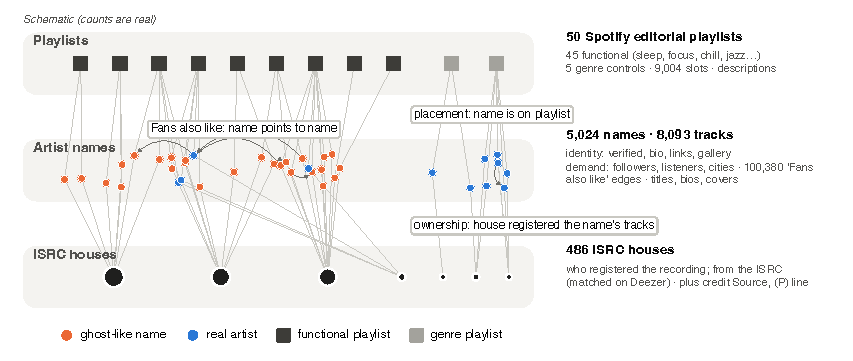
\includegraphics[width=\textwidth]{fig1_data.pdf}
\caption{\textbf{Where the playlist slots go.} Each band is a count from the data, and its width is the number of playlist slots. The left column shows the \nPlaylists{} playlists, grouped by what they are for. The middle column shows whether the name on the slot is ghost-like (orange) or real (blue). The right column shows which company registered the recording, read from its ISRC code. Companies are numbered by how many mood-playlist slots they registered. ``No recording code'' means the track was not found on Deezer.}
\label{fig:data}
\end{figure*}

% =====================================================================================
\section*{Data and how we flag a ghost-like name}

\textbf{Data.} Spotify's official API no longer lets new apps see its editorial playlists or related artists~\cite{spotify2024api}. We therefore collected one snapshot through the web player on 4 November 2026. We picked \nFunctional{} \emph{mood} playlists by hand, covering Spotify's sleep, focus, calm, jazz and classical categories. As a control we added \nGenre{} \emph{genre} playlists with well-known real artists, such as \emph{Rap UK} and \emph{ALT NOW}. Together the playlists have \nSlots{} slots holding \nTracks{} different tracks by \nNames{} artist names, since some tracks appear on more than one playlist. For every track we have the credits, the ``Source'' (the label named in the credits), the cover art (\nCovers{} covers) and, when available, a 30-second preview. For every name we have the profile (verified badge, bio, links, photos, followers, monthly listeners, top cities) and its ``Fans also like'' list of up to 20 similar artists, which gives \nFal{} links in total.

We looked up each track on Deezer to get its ISRC. This is an international recording code, and its first five characters tell who registered the recording. We call that company the \emph{house}. A name's house is the one that registered most of its tracks. Deezer found \deezerMatchF{} of the tracks on mood playlists and \deezerMatchG{} of those on genre playlists. This means \lfNoCodeF{} of mood-playlist slots have no code. Figure~\ref{fig:data} shows how all the pieces fit together.

\textbf{The flag.} We call a name \emph{ghost-like} if it is missing at least four of five signs of a public identity. These are a verified badge, a bio, a link to an outside website, a photo in the gallery, and a Spotify ``This Is'' playlist, which Spotify only makes for established artists. All other names we call \emph{real}. The rule uses nothing about who made the music or how people listen to it. So if flagged names turn out to share something there, it is a finding and not something we built in. The rule flags \nGhost{} of the \nNames{} names.

\textbf{How often is the flag wrong?} We tested the flag on four groups of names where we already know what the answer should be (Fig.~\ref{fig:checks}). None of them were used to build it. For comparison, it flags \ghostShareNamesF{} of all names on the mood playlists.

\emph{Known ghost names.} Firefly Entertainment is the company from the DN story. The flag catches \refFirefly{} of its \nFirefly{} names, so it finds most of the names it should find.

\emph{Known real artists.} It flags only \refGenreNames{} of the \nGenreNames{} artists on the genre playlists. The \nGenreFlagged{} it does flag are real musicians with thin profiles, mostly on \emph{Desi Indie}.

\emph{Classical musicians.} This is the flag's largest mistake. It flags \refMajors{} of the \nMajors{} names from Deutsche Grammophon, Decca, Sony and Warner, because orchestras and soloists hired for a recording often have no profile either. This mistake makes our results weaker, not stronger: these names are spread over many small houses, not the eight large ones.

\emph{A company with open names.} Epidemic Sound produces the same kind of background music, but releases some of it under names with a public profile. Of the \nEpidemic{} names on its own label, \epidemicBio{} have a bio, so the flag marks only \refEpidemic{}. That is the right answer, because the flag asks whether a name has a public identity, not who made the music. Two signs the flag does not use agree: half of these names' tracks credit a composer, and they have \epidemicFplRatio$\times$ as many followers per listener as a typical mood-playlist name. Epidemic's other label, Overtone Studios, is different: the flag marks 91\% of its 194 names. The same company thus releases music under both open and ghost-like names.

\textbf{Why this rule.} We chose the rule for three reasons. It only uses what any listener can see on an artist's page. It fits in one sentence, so every flag can be checked by hand. And it leaves out everything we want to test, namely who made the music, how people listen to it, and how it is recommended. If the flag used listening or production data, a finding like ``ghost-like names have no fans'' would be true by construction. The cost is that the rule makes mistakes in both directions. It flags some real musicians with thin profiles, like the classical names above. And it misses ghost-like names that have a short mood bio and a photo. In fact \realLowFpl{} of the names it calls real listen like ghosts, with a few hundred followers for up to a million listeners, and they come from the same large houses. We do not fix these mistakes with listening data, for the reason just given. Both mistakes work against our results, because the missed names sit in the largest houses and the wrongly flagged ones sit in small houses. If we did correct both using followers per listener, the share of mood-playlist slots held by ghost-like names would rise from \slotGhostF{} to \sensFplSlots{}. Where we draw the line matters more. Requiring three missing signs gives \sensThreeSlots{} and requiring all five gives \sensFiveSlots{}. But the first also flags \sensThreeMajors{} of the classical-label names, and the second catches only \sensFiveFirefly{} of Firefly's names. Every result points the same way under each version, and the house concentration in Results section 2 does not use the flag at all.

% =====================================================================================


\begin{figure}[tb]
\centering
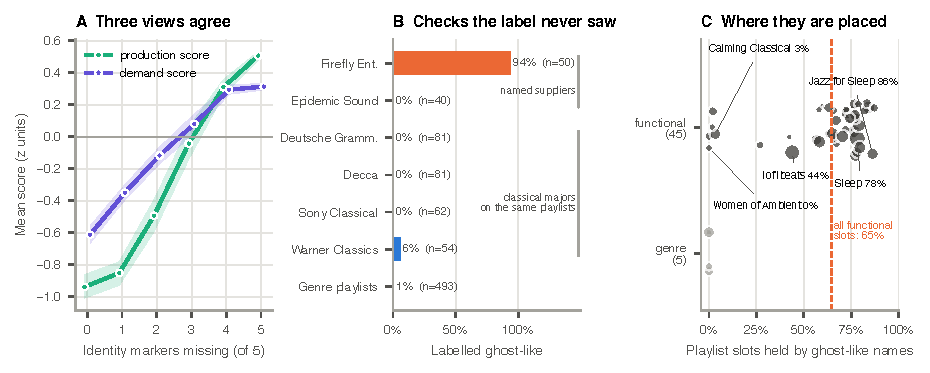
\includegraphics[width=\linewidth]{fig2_convergence.pdf}
\caption{\textbf{The flag passes tests it was not built from.} Share of names flagged ghost-like in four groups, matched by the label named in the credits. The dashed line shows the share for all names on the mood playlists.}
\label{fig:checks}
\end{figure}

\begin{figure*}[t]
\centering
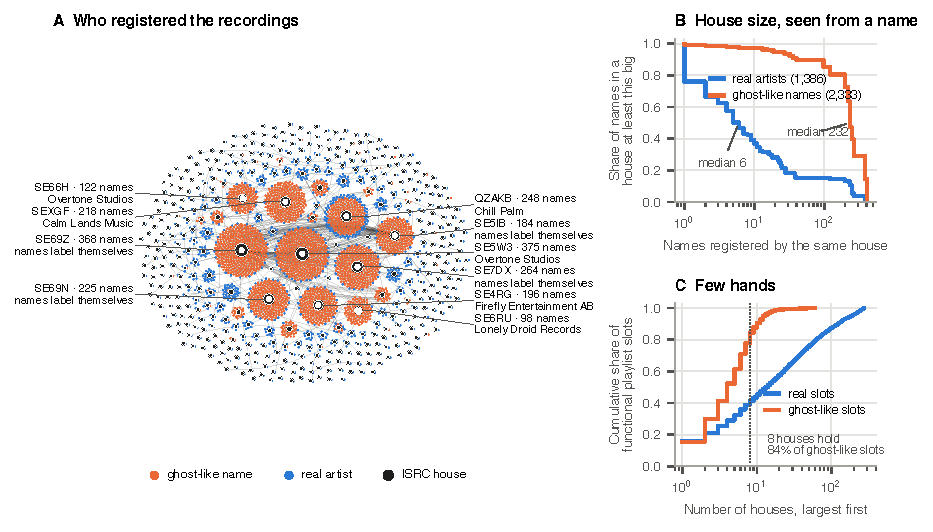
\includegraphics[width=\linewidth]{fig3_ownership.pdf}
\caption{\textbf{Hundreds of artist names, eight houses.} (\emph{A}) Each dark node is a house, and the dots around it are the artist names whose tracks it registered. The area of each disc therefore shows how many names the house has. Houses are numbered as in Fig.~\ref{fig:data}. Blue dots inside the large houses are names that happen to have a bio, but in every other way they look like their neighbours. (\emph{B}) Share of playlist slots by who registered the track, split into the eight largest houses for each kind of playlist, all other houses, and no code. Panel B does not use the ghost-like flag.}
\label{fig:ownership}
\end{figure*}

\section*{Results}

\subsection*{1. Three out of four mood-playlist slots go to ghost-like names}
Ghost-like names fill \slotGhostF{} of the slots on the \nFunctional{} mood playlists, but only \slotGhostG{} of the slots on the genre playlists (Fig.~\ref{fig:data}). Their tracks on these playlists have been played \playsGhost{} billion times in total, compared with \playsReal{} billion for the real artists next to them. The only exceptions are classical and ambient playlists built around real artists, such as \emph{Calming Classical} and \emph{Women of Ambient}.

Flagged names also differ from real artists on the \emph{same} playlists in ways the flag never looked at (Table~\ref{tab:profile}). They share their house with hundreds of other names, they have almost no followers compared with how many listeners they get, and their tracks rarely credit a real person.

\begin{table}[tb]
\centering
\caption{Ghost-like and real names on the same mood playlists. None of these numbers are used to flag a name.}
\label{tab:profile}
\begin{tabular}{lrr}
 & Ghost-like & Real \\
\midrule
Names & \profGN & \profRN \\
Other names in the same house (median) & \profGHouse & \profRHouse \\
Followers per 1{,}000 listeners (median) & \profGFpl & \profRFpl \\
Tracks that credit no person & \profGAlias & \profRAlias \\
Name listed as its own label & \profGSelf & \profRSelf \\
\bottomrule
\end{tabular}
\end{table}

\emph{What this captures and misses.} The flag measures a missing public identity, not bad intent. Some ghost-like names are simply pseudonyms of working musicians. The flag also misses ghost-like names with a short mood bio, so our shares are on the low side (see \emph{Why this rule}). The shares hold for these \nFunctional{} hand-picked playlists and would change with a different selection.

\begin{figure*}[t]
\centering
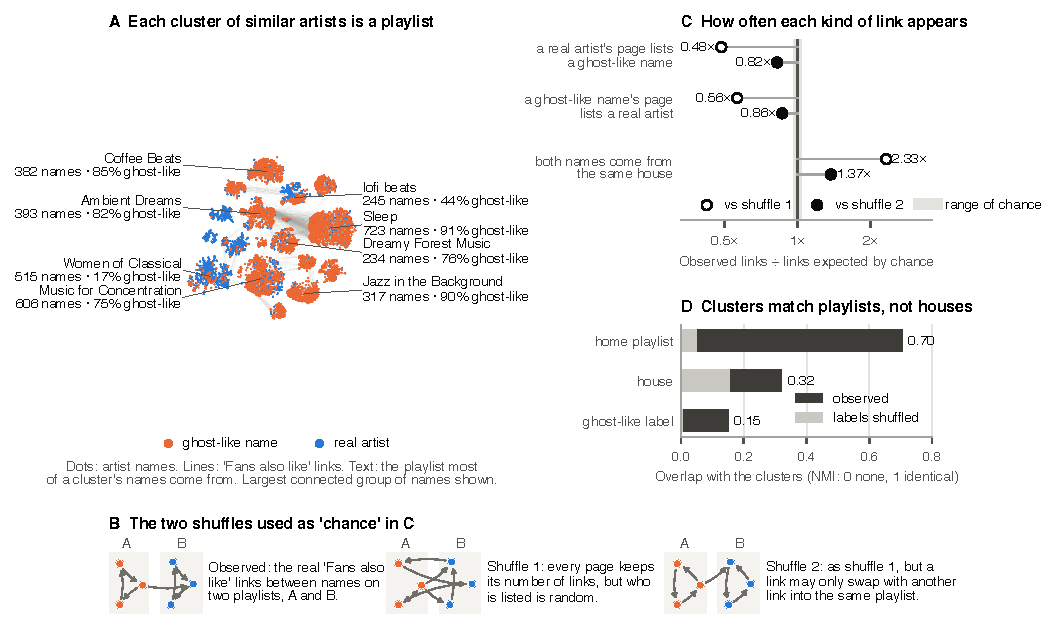
\includegraphics[width=\linewidth]{fig4_recommender.pdf}
\caption{\textbf{The recommender's map of similar artists is really a map of the playlists.} (\emph{A}) ``Fans also like'' links between the names in our data (largest connected group, \nGiant{} names), laid out by cluster. Each numbered cluster is named after the home playlist that most of its names come from, where a name's \emph{home playlist} is the playlist on which it has the most slots. The percentage is the share of ghost-like names in the cluster. (\emph{B}) The two shuffles we use to see what chance would give. (\emph{C}) Number of links of each kind that we observe, divided by the number we would expect under each shuffle (1,000 shuffles each). Chance varies by less than $\pm$\nullRange{} around 1$\times$, too little to draw. (\emph{D}) How well the clusters in A match three ways of grouping the names (home playlist, house and ghost-like flag), measured by normalised mutual information. Grey bars show the same score when the grouping is shuffled.}
\label{fig:recommender}
\end{figure*}

\subsection*{2. The credits show hundreds of artists, but the recording codes show eight houses}
In the credits, ghost-like names look self-released. \selfSourceGhost{} of them list \emph{their own name} as the label of their tracks, compared with \selfSourceReal{} of the real artists on the same playlists. The credits are the only place a listener can check who made a track, and there each of these names looks like an independent musician. The recording codes tell a different story. The names that list themselves as their own label sit in houses with a median of \selfSourceHouse{} other names.

Figure~\ref{fig:ownership}A shows the network of names and houses. Of the \ghostWithReg{} ghost-like names with a recording code, \topEightGhostNames{} come from just eight houses, and \topEightSE{} of those eight use Swedish codes. Across all ghost-like names with a code, \seGhost{} have a Swedish one, compared with \seReal{} of the real artists. This fits the press reports about Swedish production companies~\cite{ingham2022mbw,stassen2024mbw}. For four of the eight houses, no company is named anywhere in the credits. Two belong to Overtone Studios, which is owned by Epidemic Sound~\cite{stassen2024mbw}, and one is Firefly Entertainment.

This concentration does not depend on our flag. If we simply count every mood-playlist slot by the code on its track, the eight largest houses registered \lfTopEightCodedF{} of the slots that have a code. On the genre playlists, the eight largest houses registered only \lfTopEightCodedG{} (Fig.~\ref{fig:ownership}B).

\emph{What this captures and misses.} A house is whoever registered the recording. That can be a label or a distributor, and not necessarily the composer. \nMultiHouse{} names have tracks in more than one house, often the same pair of large houses, so the eight houses may in fact be fewer than eight companies.





\begin{figure*}[tb]
\centering
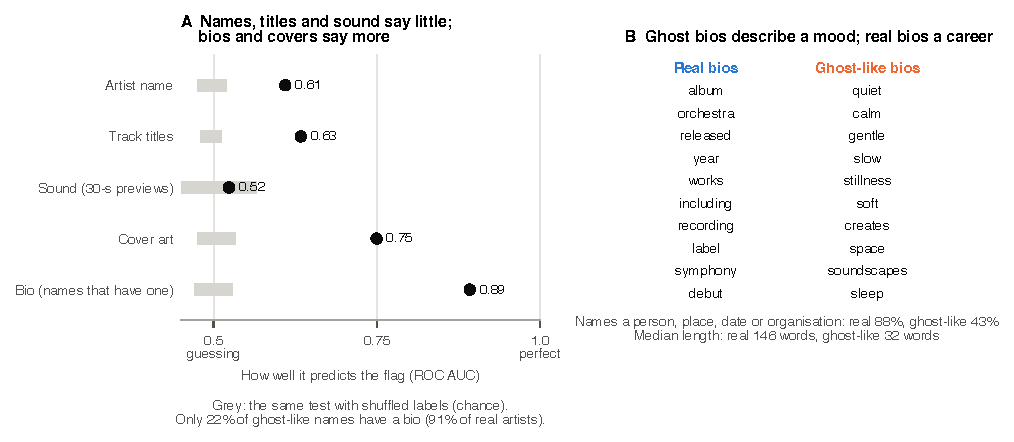
\includegraphics[width=0.95\linewidth]{fig5_text.pdf}
\caption{\textbf{What a listener sees.} (\emph{A}) How well each kind of visible content predicts the ghost-like flag among mood-playlist names, measured as cross-validated ROC AUC. (\emph{B}) The words most typical of ghost-like bios and of real bios (weighted log-odds~\cite{monroe2008fightin}).}
\label{fig:text}
\end{figure*}

\subsection*{3. The recommender does not push listeners to ghosts, it mirrors the playlists}
Every artist page lists up to 20 ``Fans also like'' artists. These lists show who the recommender thinks is similar to whom, and \nFalIn{} of the links point to another name in our data. On real artists' pages, \realSlotsToGhost{} of the recommendations are ghost-like names. On ghost-like names' pages, \ghostSlotsToGhost{} are other ghost-like names.

To see if this is more or less than chance, we compared the real links with two shuffled versions of the same network (Fig.~\ref{fig:recommender}B). In \emph{shuffle 1}, every page keeps its number of links, but which artists are listed is random. In \emph{shuffle 2}, a link can only be swapped with another link that points into the same playlist, so the playlist structure is kept.

Compared with shuffle 1, real artists list ghost-like names only \flowRGDeg$\times$ as often as chance would give, and ghost-like names list real artists \flowGRDeg$\times$ as often (Fig.~\ref{fig:recommender}C). We had expected a ``funnel'', where real artists send listeners on to ghosts but ghosts rarely send them back. We found no funnel. Both directions are reduced by about the same amount. Most of this separation comes from the playlists. Compared with shuffle 2, the numbers move to \flowRGPl$\times$ and \flowGRPl$\times$. In other words, people who found a name on \emph{Sleep} also listen to other names on \emph{Sleep}.

So ghost-like names do not get their listeners from the recommender. They get them from the playlists. Spotify shows, for each artist, the playlist where most of their listeners found them. For \discOursG{} of ghost-like names this is one of our editorial playlists, compared with \discOursR{} of the real artists next to them. Ghost-like names also live in a closed neighbourhood. \inSetGhost{} of the links on their pages point to other names in our data, compared with \inSetReal{} for real artists, whose recommendations reach out to artists outside the playlists we collected.

One pattern goes beyond the playlists. Names from the same house are linked \samePl$\times$ as often as shuffle 2 predicts (\sameObs{} links against \sameExpPl{} expected).

Clustering the network shows which of the two effects is stronger. The Louvain method~\cite{blondel2008louvain} finds \nComm{} clusters (Fig.~\ref{fig:recommender}A). These clusters match each name's home playlist (the playlist on which the name has the most slots) closely, with a normalised mutual information of \nmiHome{} (\nmiHomeNull{} when shuffled). They match the house much less, at \nmiHouse{} (\nmiHouseNull{} when shuffled) (Fig.~\ref{fig:recommender}D). So the playlists shape the recommender's map, and houses add a smaller pull on top, which the count above picks out. Even part of that house effect comes from the playlists, since a house's names tend to sit on the same few playlists.

\emph{What this captures and misses.} ``Fans also like'' is what the recommender outputs, not how it works inside. We therefore cannot say why names from the same house are linked. Shared composers and a shared sound could make people listen to them together without the recommender treating houses in any special way. What the result does show is that playlist placement creates shared listening, and shared listening then becomes ``similarity''.

% =====================================================================================


\subsection*{What a listener sees}
Would a listener notice? A listener sees an artist's name, track titles, cover art, the music itself and sometimes a bio. We asked how much each of these gives away on its own. For each kind of content we trained a simple classifier to predict the flag, and tested it on names it had not seen (Fig.~\ref{fig:text}A). We report the ROC AUC. This is the chance that the classifier ranks a random ghost-like name above a random real one, so 0.5 means guessing and 1 means perfect. We only used names from mood playlists, so the classifier cannot cheat by telling sleep music apart from rap.

\emph{Names and titles.} The text classifiers look for short pieces of words (for names) or for words and word pairs (for titles and bios) that are more common in one group than the other. Artist names give an AUC of \aucName, which is close to guessing. Ghost-like names are made to look like real people. \personGhost{} of them are a two-word ``Firstname Lastname'', exactly as many as for the real artists next to them (\personRealF). Track titles do a little better (\aucTitles). Ghost-like titles are slightly shorter (\titleWordsGhost{} words against \titleWordsReal), but other names reuse them about as often as they reuse real titles (\titleReuseGhost{} against \titleReuseReal).

\emph{Sound and covers.} The music itself gives nothing away. We described \nAudio{} 30-second previews by tempo, loudness, brightness and timbre, and a classifier on these gets \aucAudio{}, no better than chance. On the same playlist, ghost tracks sound just like real ones. Cover art does better (\aucCover), and the covers have a house style. If we take a cover and find the most similar cover under \emph{another} name, it comes from the same house \coverSameHouse{} of the time, against \coverSameHouseNull{} by chance.

\emph{Bios.} Bios give away the most (AUC \aucBio), but only \bioGhost{} of ghost-like names have one, compared with \bioReal{} of real artists. Much of the signal is length alone. Bio length by itself reaches \aucBioLength, because ghost bios have a median of \tokGhost{} words and real bios \tokReal. The words also differ. We ranked words by how much more often they appear in one group's bios than in the other's, adjusted so that rare words do not take over (weighted log-odds~\cite{monroe2008fightin}). Ghost bios describe a mood, with words like \emph{quiet}, \emph{calm} and \emph{stillness}. Real bios describe a career, with words like \emph{album}, \emph{released} and \emph{debut} (Fig.~\ref{fig:text}B). Many real artists on these playlists are classical, so words like \emph{orchestra} and \emph{symphony} also show up. Finally, we used named-entity recognition, which finds people, places, dates and organisations in a text. At least one such entity appears in \entReal{} of real bios but in only \entGhost{} of ghost-like ones. A real bio tells a life story, while a ghost bio describes an atmosphere.

In short, the things a listener notices first, namely the name, the titles and the sound, look the same for both groups. Only the rarer clues, a written bio and to a lesser extent the cover, set them apart.

% =====================================================================================
\section*{Discussion}
Three out of four slots on Spotify's mood playlists go to names with no public identity. The credits make them look self-released, but their recording codes lead back to a small number of houses, most of them Swedish. The press needed leaked lists to show this. We show that public recording codes are enough. Spotify's recommender does not funnel listeners from real artists to these names. Its idea of similarity mostly copies its own playlists, and on top of that, names from the same house stick together. A listener can hardly tell the difference, because the names, titles and sound look like those of real artists.

These results suggest where to look next. If you want to know who is behind a playlist, recording codes are a free and public way to check. Anyone can repeat our ownership analysis for another country or another month. If you want to know how catalogue music reaches listeners, look at how playlists are put together, not at the recommender, which mostly echoes the playlists. As AI makes this kind of music even cheaper to produce, the same two tools could show how fast it spreads.

\emph{Limitations.} This is a single snapshot. Daily snapshots would show whether ghost-like names replace real artists over time. The playlists are Spotify's global playlists as seen from Denmark, and we did not test whether their track lists differ between countries. The flag misses suppliers with real-looking profiles and wrongly flags some classical names. Deezer fails to find mood-playlist tracks more often than genre tracks, so houses are measured on only \deezerMatchF{} of them, and one large supplier is almost missing from Deezer. House sizes are counted within our sample only.

\emph{Ethics.} Spotify's terms do not allow automated collection, so we kept our data collection small and slow. We downloaded no audio from Spotify and only used Deezer's official previews, which we processed locally. Some ghost-like names belong to real musicians, so we report houses and companies as groups and never profile named individuals.

% =====================================================================================
\matmethods{
\textbf{Collection.} On 4 November 2026 we queried Spotify's web-player API from an anonymous session in Denmark, at about 10 requests per second. Of the 2,622 Spotify-owned playlists on the Danish browse page, we kept the editorial playlists that are the same for every listener. From these we picked \nFunctional{} mood and \nGenre{} genre playlists by hand. We matched tracks to Deezer's public API by artist and title, and checked that the durations agree. The matches are reliable, since titles agree exactly for over 99\% of tracks and the artist always matches. The house is the first five characters of the ISRC (country and registrant code). A house's size is the number of names that have it as their house.

\textbf{Shuffles.} The network has a directed link from each name to every name in our data that appears on its ``Fans also like'' list (\nFalIn{} links). Shuffle 1 randomly reassigns the targets of all links, which keeps every name's number of outgoing and incoming links. This is a directed configuration model~\cite{maslov2002specificity}. Shuffle 2 only reassigns targets among links whose target has the same home playlist, meaning the playlist where the name has most slots. We report the observed counts divided by the average over 1,000 shuffles.

\textbf{Clusters.} We ran Louvain~\cite{blondel2008louvain} on the undirected network using igraph~\cite{csardi2006igraph}. It gives a modularity of $Q=\louvainQ$, against \louvainQnull{} for networks rewired with the same degrees~\cite{guimera2004modularity}. We compare normalised mutual information~\cite{danon2005nmi} with 100 shuffles of the grouping. The layouts use Fruchterman and Reingold's method~\cite{fruchterman1991} inside each cluster and are only for display.

\textbf{Text, images and sound.} The classifiers use TF-IDF with logistic regression~\cite{pedregosa2011sklearn}. For names we use pieces of 2 to 4 characters, and for titles and bios we use single words and word pairs, with the artist's own name removed. We test with 5-fold stratified cross-validation and use 20 runs with shuffled labels as the chance level. Named entities come from spaCy~\cite{honnibal2020spacy}. Cover embeddings come from OpenCLIP ViT-B/32~\cite{radford2021clip,cherti2023openclip}, averaged per artist. Audio features (tempo, loudness, brightness, timbre) were computed with librosa~\cite{mcfee2015librosa} on \nAudio{} Deezer previews from \nAudioPlaylists{} playlists.

\textbf{Reproducibility.} Every number in this paper is written by \texttt{src/paper\_numbers.py} from the processed data, and every figure is made by one script in \texttt{src/figures/}. All random seeds are fixed.
}

\showmatmethods{} % Display the Materials and Methods section

\dataavail{Code and processed data are available at \url{https://github.com/Benyla/02805_SGI} (folder \texttt{project/}).}

\acknow{We thank the teaching staff of 02805 Social Graphs and Interactions at DTU for feedback on this project.}

\showacknow{} % Display the acknowledgments section

% Author contributions, share of each part (rows sum to 100%).
\vskip 2ex plus 1ex minus .5ex
\noindent{\sffamily\bfseries\fontsize{7}{9}\selectfont AUTHOR CONTRIBUTIONS.}\par\vskip 0.5ex
{\small\noindent
\begin{tabular*}{\columnwidth}{@{\extracolsep{\fill}}lrrr}
\toprule
Part & A.H.J. & B.N.L. & S.B. \\
\midrule
Data collection & 20\% & 60\% & 20\% \\
Ghost-like flag (identity markers) & 30\% & 45\% & 25\% \\
Playlist placement (Results 1) & 25\% & 25\% & 50\% \\
Ownership network (Results 2) & 20\% & 30\% & 50\% \\
Recommender audit (Results 3) & 50\% & 20\% & 30\% \\
Text, covers and audio & 60\% & 20\% & 20\% \\
Introduction and Discussion & 25\% & 35\% & 40\% \\
\bottomrule
\end{tabular*}\par}
\vskip 2ex

% No \bibsplit here. It forces a column break inside the reference list,
% which leaves white space on the last page and overlaps the table above.

% Bibliography
\bibliography{refs}

\end{document}
